\documentclass[11pt]{article}
\usepackage{geometry}
\usepackage{tcolorbox}
\usepackage{hyperref}
\usepackage{microtype}
\usepackage{XCharter}
\usepackage{rotating}
\usepackage[backend=biber,sorting=none,style=apa]{biblatex}
\addbibresource{library.bib}
\geometry{
    a4paper,
    total={170mm,257mm},
    left=20mm,
    top=20mm,
}
\setlength{\parskip}{5pt}
\setlength\parindent{0pt}
\usepackage{graphicx}
\usepackage{booktabs}
\usepackage{subcaption}
\usepackage{amsmath}
\usepackage{amsfonts}
\usepackage{amssymb}
\usepackage{lscape}
\usepackage{psfrag}
\usepackage{hyperref}
\hypersetup{
  colorlinks = false,
  urlcolor   = blue,
  linkcolor  = blue,
  citecolor  = red
}
\usepackage{verbatim}
\usepackage{textcomp}
\usepackage{multirow}
\usepackage{rotating}
\usepackage{adjustbox}
\usepackage{tikz}
\usepackage[english]{babel}
\usepackage{appendix}
\usepackage{parskip}
\usepackage{placeins}
\usepackage[tableposition=top]{caption}
\sloppy
\widowpenalty=10000
\clubpenalty=10000
\edef\today{%\number\day\
\ifcase\month\or
January\or February\or March\or April\or May\or June\or July\or
August\or September\or October\or November\or December\fi\ \number\year}
\title{\vspace*{40.0mm}
  \bf\sf Assignment
         \vspace*{20.0mm} \\
  \vspace*{40.0mm}}
\author{\sf Van den Broeck Sebastiaan (r0902562)}
\date{\sf 13/03/2023}

\begin{document}

\begin{figure}
  \parbox[t]{125mm}{
    \vspace*{6mm}
    \scriptsize\sf           FACULTY OF SCIENCE \\
    \scriptsize\sf           DEPARTMENT OF MATHEMATICS \\
    \scriptsize\sf\bfseries  MASTER OF STATISTICS AND DATA SCIENCE \\
    \scriptsize\sf\bfseries  STRUCTURAL EQUATION MODELING \\}
  \parbox[t]{40mm}{
    \begin{flushright}
      
\includegraphics[height=15mm]{logo.eps.pdf}
    \end{flushright}}
\end{figure}

\maketitle
\thispagestyle{empty}
\raggedbottom

\cleardoublepage
\setcounter{page}{1}
\setcounter{tocdepth}{3}

\section{Introduction}

Harm avoidance and self-directedness have been linked to depression.
A behaviour can be classified under harm avoidance if it is done to avoid novelty and punishment.
Self-directedness, on the other hand, is a form of self-determination and ability to regulate behaviour to suit goals and values.
It has been proposed that harm avoidance and self-directedness are indirectly linked to depression through social functioning (\cite{tse2011}).
In this work I will test this hypothesis on a new dataset, which will be discussed next.
A structural equation model has been used to test the hypothesis and will be discussed next.
Lastly, the results and implications thereof will be considered.

\section{Data}

The data treated in the report is the Midlife in the United States (MIDUS) series.
Currently, there are three waves in the study, which were collected via phone interviews, surveys and by bringing participants into clinical settings to facility collecting biological data.
All three waves cover the contiguous United States in its entirety.
The first wave was collected in 1995 and 1996, while the second wave was collected in 2004 and 2005.
The most recent wave was collected in 2013 and 2014.
The second and third wave have been combined to create a bigger dataset.
It was not possible to incorporate the first dataset, since a lot of variables changed between the first and second and third waves (\cite{radler2014}).

An important reason for choosing this dataset is that it contains a lot of documentation for which variables form certain latent constructs such as depression or social anxiety.
Since I am not familiar with the field of psychology this would save me a lot of time.
Depression is the most important latent variable in this work.
It has been measures through seven questions during which the respondent reflects over the last two weeks.
For example, the questions include losing interest, becoming tired, having trouble falling asleep or thinking about death.
Each variable which measures this latent construct has been coded such that a 1 reflects a yes answer.
As could be expected, a 0 then means a respondent has answered no.

\begin{table}[h!]
\scalebox{0.8}{
\begin{tabular}{|l|l|l|}
\hline
\textbf{Construct}          & \textbf{Code} & \textbf{Question}                                                                                                                                              \\ \hline
\multirow{7}{*}{Depression} & PA63        & During those two weeks, did you lose interest in most things?                                                                                                  \\ \cline{2-3} 
                            & P164        & \begin{tabular}[c]{@{}l@{}}Thinking about these same two weeks, did you feel more tired\\ out or low on energy?\end{tabular}                                   \\ \cline{2-3} 
                            & PA65        & During those same two weeks, did you lose appetite?                                                                                                            \\ \cline{2-3} 
                            & PA66        & \begin{tabular}[c]{@{}l@{}}Did you have more trouble falling asleep than you usually do\\ during those two weeks?\end{tabular}                                 \\ \cline{2-3} 
                            & PA67        & \begin{tabular}[c]{@{}l@{}}During that same two week period, did you have a lot more\\ trouble concentrating than usual?\end{tabular}                          \\ \cline{2-3} 
                            & PA68        & \begin{tabular}[c]{@{}l@{}}People sometimes feel down on themselves, no good, or worthless.\\ During that two-week period, did you feel this way?\end{tabular} \\ \cline{2-3} 
                            & PA69        & \begin{tabular}[c]{@{}l@{}}Did you think a lot about death - either your own, someone else's\\ or death in general - during those two weeks?\end{tabular}      \\ \hline
\end{tabular}
}
\end{table}

\begin{table}[h]
\scalebox{0.8}{
\begin{tabular}{|l|l|ll|}
\hline
\multirow{2}{*}{\textbf{Construct}} & \multirow{2}{*}{\textbf{Code}} & \multicolumn{2}{l|}{\textbf{Count}} \\ \cline{3-4} 
                                    &                                & \multicolumn{1}{l|}{0}      & 1     \\ \hline
\multirow{7}{*}{Depression}         & PA63                         & \multicolumn{1}{l|}{156}    & 633   \\ \cline{2-4} 
                                    & P164                         & \multicolumn{1}{l|}{61}     & 726   \\ \cline{2-4} 
                                    & PA65                         & \multicolumn{1}{l|}{338}    & 445   \\ \cline{2-4} 
                                    & PA66                         & \multicolumn{1}{l|}{223}    & 565   \\ \cline{2-4} 
                                    & PA67                         & \multicolumn{1}{l|}{111}    & 675   \\ \cline{2-4} 
                                    & PA68                         & \multicolumn{1}{l|}{283}    & 507   \\ \cline{2-4} 
                                    & PA69                         & \multicolumn{1}{l|}{304}    & 485   \\ \hline
\end{tabular}
}
\end{table}

Another important aspect in this report is harm avoidance. Since it cannot be measured directly, four questions were asked to get an idea about this variable.
First, interviewees were asked whether they would enjoy experiencing an earthquake or learning to walk the tightrope.
These two variables were reverse recoded such that a 4 reflects not agreeing with the statement at all (harm avoidance), while a 1 indicates fully agreeing (no avoidance).
Second, interviewees were presented with two scenario's twice.
For each question, one scenario corresponds to a harmful situation, while the other scenario's is harmless.
Again, there was a recoding such that a higher score on these two variables indicates avoiding harm.

\begin{table}[h!]
\scalebox{0.8}{
\begin{tabular}{|l|l|l|}
\hline
\textbf{Construct}              & \textbf{Code} & \textbf{Question}                                                                                                                                                                                                                                                                                                              \\ \hline
\multirow{4}{*}{Harm avoidance} & SE7D        & It might be fun and exciting to be in an earthquake.                                                                                                                                                                                                                                                                           \\ \cline{2-3} 
                                & SE7V        & It might be fun learning to walk a tightrope.                                                                                                                                                                                                                                                                                  \\ \cline{2-3} 
                                & SE8         & \begin{tabular}[c]{@{}l@{}}Of these two situations, I would dislike more: Situation 1: \\ Riding a long stretch of rapids in a canoe; Situation 2:\\ Waiting for someone who's late.\end{tabular}                                                                                                                              \\ \cline{2-3} 
                                & SE9         & \begin{tabular}[c]{@{}l@{}}Of these two situations, I would dislike more: Situation 1:\\ Being at the circus when two lions suddenly get loose\\ down in the ring; Situation 2: Bringing my whole family\\ to the circus and then not being able to get in because a\\ clerk sold me tickets for the wrong night.\end{tabular} \\ \hline
\end{tabular}
}
\end{table}

\begin{table}[h!]
\scalebox{0.8}{
\begin{tabular}{|l|l|llll|}
\hline
\multirow{2}{*}{\textbf{Construct}} & \multirow{2}{*}{\textbf{Code}} & \multicolumn{4}{l|}{\textbf{Count}}                                                                              \\ \cline{3-6} 
                                    &                                & \multicolumn{1}{l|}{\textbf{1 (harm)}} & \multicolumn{1}{l|}{\textbf{2}} & \multicolumn{1}{l|}{\textbf{3}} & \textbf{4 (no harm)} \\ \hline
\multirow{2}{*}{Harm avoidance}     & SE7D                         & \multicolumn{1}{l|}{274}               & \multicolumn{1}{l|}{875}        & \multicolumn{1}{l|}{838}        & 4889                 \\ \cline{2-6} 
                                    & SE7V                         & \multicolumn{1}{l|}{367}               & \multicolumn{1}{l|}{1222}       & \multicolumn{1}{l|}{1163}       & 4238                 \\ \hline
\end{tabular}
}
\end{table}

\begin{table}[h!]
\scalebox{0.8}{
\begin{tabular}{|l|l|ll|}
\hline
\multirow{2}{*}{\textbf{Construct}} & \multirow{2}{*}{\textbf{Code}} & \multicolumn{2}{l|}{\textbf{Count}}          \\ \cline{3-4} 
                                    &                                & \multicolumn{1}{l|}{\textbf{0 (harm)}} & \textbf{1 (no harm)} \\ \hline
\multirow{2}{*}{Harm avoidance}     & SE8                          & \multicolumn{1}{l|}{3803}                 & 3089       \\ \cline{2-4} 
                                    & SE7V                         & \multicolumn{1}{l|}{2994}                 & 3898       \\ \hline
\end{tabular}
}
\end{table}

We should not forget about self-directedness, which has been measured through three variables.
Making plans for the future, knowing what to want out of life and setting goals are important for this dimension.
Again, the variables were reverse coded such that a higher score reflects agreeing more with the statement.
The data indicates that most participants agree somewhat or fully what the three statements.

\begin{table}[h!]
\scalebox{0.8}{
\begin{tabular}{|l|l|l|}
\hline
\textbf{Construct}                 & \textbf{Code} & \textbf{Question}                                   \\ \hline
\multirow{3}{*}{Self-directedness} & SE14O       & I like to make plans for the future.                \\ \cline{2-3} 
                                   & SE14R       & I know what I want out of life.                     \\ \cline{2-3} 
                                   & SE14P       & I find it helpful to set goals for the near future. \\ \hline
\end{tabular}
}
\end{table}

\begin{table}[h!]
\scalebox{0.8}{
\begin{tabular}{|l|l|llll|}
\hline
\multirow{2}{*}{\textbf{Construct}} & \multirow{2}{*}{\textbf{Code}} & \multicolumn{4}{l|}{\textbf{Count}}                                                                              \\ \cline{3-6} 
                                    &                                & \multicolumn{1}{l|}{\textbf{1}} & \multicolumn{1}{l|}{\textbf{2}} & \multicolumn{1}{l|}{\textbf{3}} & \textbf{4} \\ \hline
\multirow{3}{*}{Self-directedness}  & SE14O                        & \multicolumn{1}{l|}{247}        & \multicolumn{1}{l|}{1303}       & \multicolumn{1}{l|}{2754}       & 2590       \\ \cline{2-6} 
                                    & SE14R                        & \multicolumn{1}{l|}{251}        & \multicolumn{1}{l|}{1089}       & \multicolumn{1}{l|}{2929}       & 2604       \\ \cline{2-6} 
                                    & SE14P                        & \multicolumn{1}{l|}{318}        & \multicolumn{1}{l|}{1320}       & \multicolumn{1}{l|}{3071}       & 2184       \\ \hline
\end{tabular}
}
\end{table}

Lastly, the latent variable social functioning has been used in the analysis.
Seven questions related to this dimension were asked.
The variables SE1BB, SE1D, SE1I and SE1V were reverse coded such that a higher score indicates a higher degree of social functioning.
The dataset counts 601 observations after deleting rows with missing values.

\begin{table}[h!]
\scalebox{0.8}{
\begin{tabular}{|l|l|l|}
\hline
\textbf{Construct}                  & \textbf{Code} & \textbf{Question}                                                                                                                                    \\ \hline
\multirow{7}{*}{Social functioning} & SE1BB       & \begin{tabular}[c]{@{}l@{}}People would describe me as a giving person, willing to share my time \\ with others.\end{tabular}                        \\ \cline{2-3} 
                                    & SE1D        & Most people see me as loving and affectionate.                                                                                                       \\ \cline{2-3} 
                                    & SE1HH       & I have not experienced many warm and trusting relationships with others.                                                                             \\ \cline{2-3} 
                                    & SE1J        & Maintaining close relationships has been difficult and frustrating for me.                                                                           \\ \cline{2-3} 
                                    & SE1I        & \begin{tabular}[c]{@{}l@{}}I think it is important to have new experiences that challenge how you think\\ about yourself and the world.\end{tabular} \\ \cline{2-3} 
                                    & SE1P        & \begin{tabular}[c]{@{}l@{}}I often feel lonely because I have few close friends with whom to share my\\ concerns.\end{tabular}                       \\ \cline{2-3} 
                                    & SE1V        & I enjoy personal and mutual conversations with family members and friends.                                                                           \\ \hline
\end{tabular}
}
\end{table}

\begin{table}[h!]
\scalebox{0.8}{
\begin{tabular}{|l|l|lllllll|}
\hline
\multirow{2}{*}{\textbf{Construct}} & \multirow{2}{*}{\textbf{Code}} & \multicolumn{7}{l|}{\textbf{Count}}                                                                                                                                                                                    \\ \cline{3-9} 
                                    &                                & \multicolumn{1}{l|}{\textbf{1}} & \multicolumn{1}{l|}{\textbf{2}} & \multicolumn{1}{l|}{\textbf{3}} & \multicolumn{1}{l|}{\textbf{4}} & \multicolumn{1}{l|}{\textbf{5}} & \multicolumn{1}{l|}{\textbf{6}} & \textbf{7} \\ \hline
\multirow{7}{*}{Social functioning} & SE1BB                        & \multicolumn{1}{l|}{28}         & \multicolumn{1}{l|}{76}         & \multicolumn{1}{l|}{127}        & \multicolumn{1}{l|}{472}        & \multicolumn{1}{l|}{799}        & \multicolumn{1}{l|}{2382}       & 3055       \\ \cline{2-9} 
                                    & SE1D                         & \multicolumn{1}{l|}{43}         & \multicolumn{1}{l|}{126}        & \multicolumn{1}{l|}{219}        & \multicolumn{1}{l|}{807}        & \multicolumn{1}{l|}{815}        & \multicolumn{1}{l|}{2598}       & 230        \\ \cline{2-9} 
                                    & SE1HH                        & \multicolumn{1}{l|}{291}        & \multicolumn{1}{l|}{501}        & \multicolumn{1}{l|}{575}        & \multicolumn{1}{l|}{441}        & \multicolumn{1}{l|}{497}        & \multicolumn{1}{l|}{1382}       & 3242       \\ \cline{2-9} 
                                    & SE1J                         & \multicolumn{1}{l|}{236}        & \multicolumn{1}{l|}{575}        & \multicolumn{1}{l|}{818}        & \multicolumn{1}{l|}{711}        & \multicolumn{1}{l|}{512}        & \multicolumn{1}{l|}{1524}       & 2550       \\ \cline{2-9} 
                                    & SE1I                         & \multicolumn{1}{l|}{113}        & \multicolumn{1}{l|}{136}        & \multicolumn{1}{l|}{142}        & \multicolumn{1}{l|}{709}        & \multicolumn{1}{l|}{1154}       & \multicolumn{1}{l|}{2190}       & 2483       \\ \cline{2-9} 
                                    & SE1P                         & \multicolumn{1}{l|}{242}        & \multicolumn{1}{l|}{447}        & \multicolumn{1}{l|}{744}        & \multicolumn{1}{l|}{655}        & \multicolumn{1}{l|}{479}        & \multicolumn{1}{l|}{1321}       & 3036       \\ \cline{2-9} 
                                    & SE1V                         & \multicolumn{1}{l|}{63}         & \multicolumn{1}{l|}{64}         & \multicolumn{1}{l|}{105}        & \multicolumn{1}{l|}{211}        & \multicolumn{1}{l|}{589}        & \multicolumn{1}{l|}{1879}       & 4024       \\ \hline
\end{tabular}
}
\end{table}

\begin{figure}[h!]
\centering
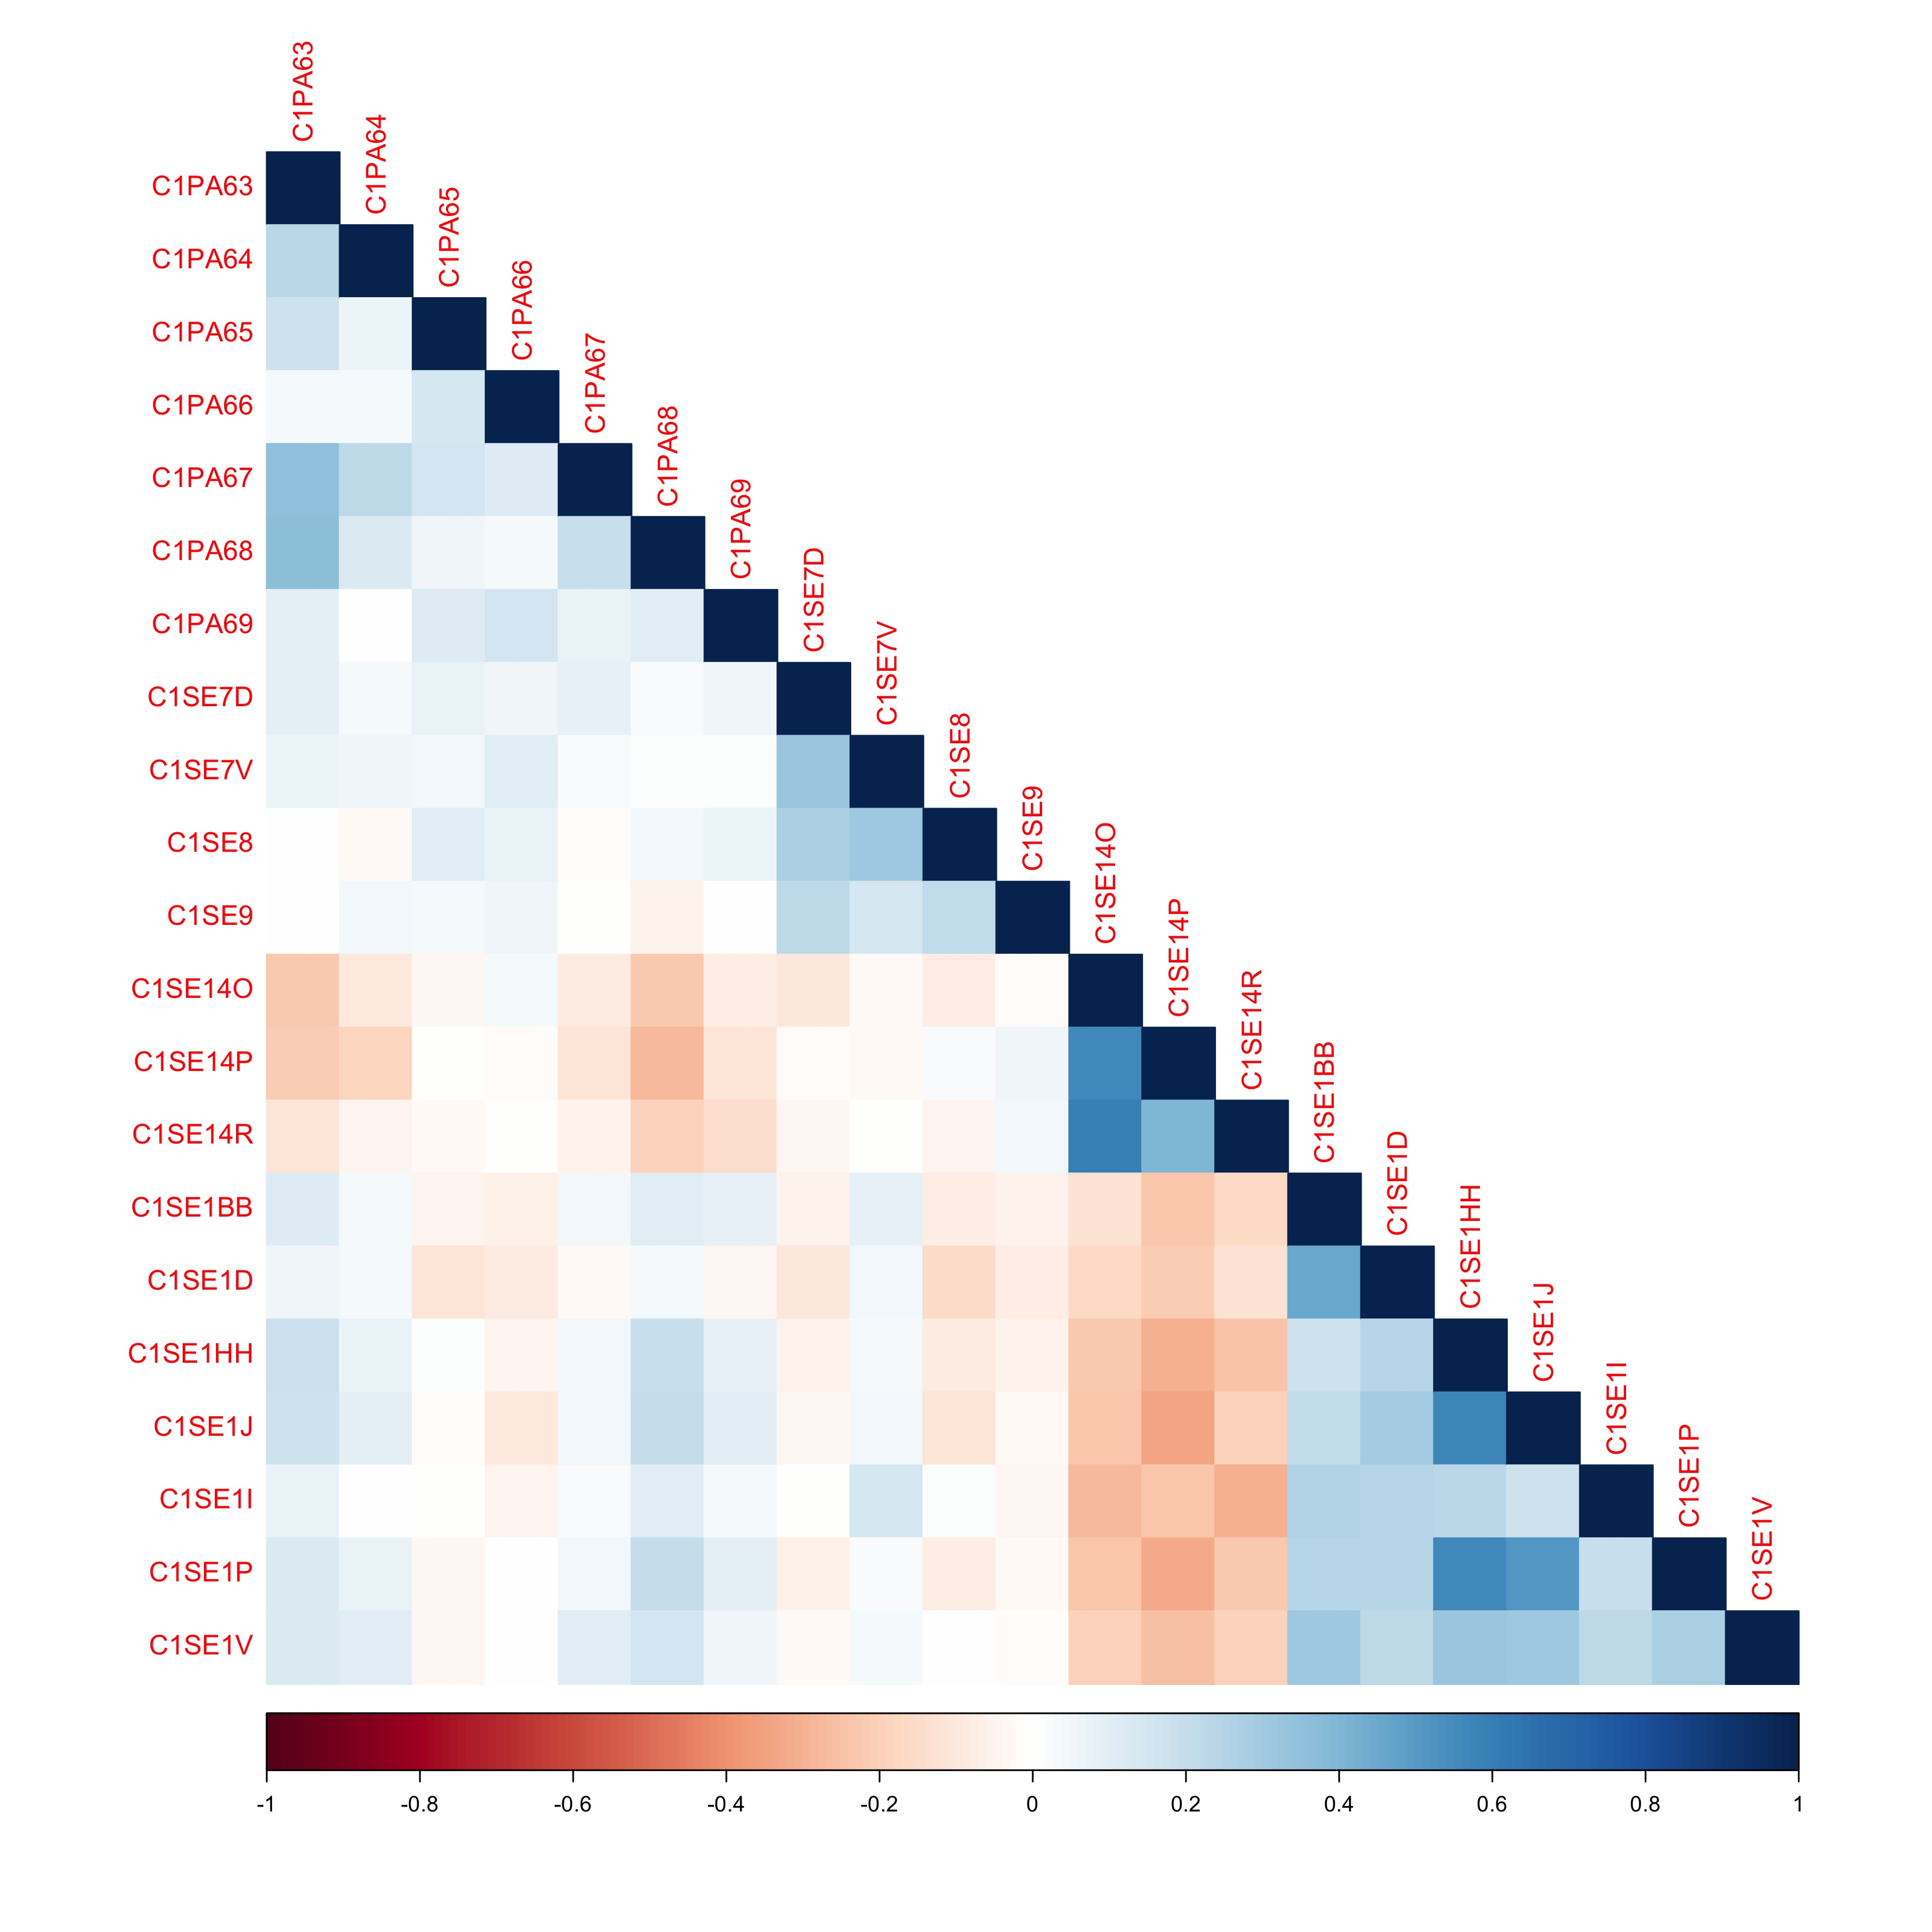
\includegraphics[width=14cm]{../visualizations/corr.png}
\caption{Correlation plot}
\end{figure}

\FloatBarrier
\pagebreak
\section{The base model}

The base model has four latent variables which are related to each other through a structural model.
Social functioning has been expressed linearly through harm avoidance and self directedness.
Depression is estimated to have a linear relationship with social functioning.
Hence, there is no direct effect of the exogenous variables harm avoidance and self directedness on depression.

\begin{equation}
    \footnotesize
    \begin{cases}
    \textrm{PA63}  & = \lambda_{11} \textrm{depression} + \delta_{11} \\
    \textrm{PA64}  & = \lambda_{12} \textrm{depression} + \delta_{12} \\
    \textrm{PA65}  & = \lambda_{13} \textrm{depression} + \delta_{13} \\
    \textrm{PA66}  & = \lambda_{14} \textrm{depression} + \delta_{14} \\
    \textrm{PA67}  & = \lambda_{15} \textrm{depression} + \delta_{15} \\
    \textrm{PA68}  & = \lambda_{16} \textrm{depression} + \delta_{16} \\
    \textrm{PA69}  & = \lambda_{17} \textrm{depression} + \delta_{17} \\
    \textrm{SE7V}  & = \lambda_{21} \textrm{harm avoidance} + \delta_{21} \\
    \textrm{SE7D}  & = \lambda_{22} \textrm{harm avoidance} + \delta_{22} \\
    \textrm{SE8}   & = \lambda_{23} \textrm{harm avoidance} + \delta_{23} \\
    \textrm{SE9}   & = \lambda_{24} \textrm{harm avoidance} + \delta_{24} \\
    \textrm{SE14O} & = \lambda_{31} \textrm{self directedness} + \delta_{31} \\
    \textrm{SE14P} & = \lambda_{32} \textrm{self directedness} + \delta_{32} \\
    \textrm{SE14R} & = \lambda_{33} \textrm{self directedness} + \delta_{33} \\
    \textrm{SE1BB} & = \lambda_{41} \textrm{social functioning} + \delta_{41} \\
    \textrm{SE1D}  & = \lambda_{42} \textrm{social functioning} + \delta_{42} \\
    \textrm{SE1HH} & = \lambda_{43} \textrm{social functioning} + \delta_{43} \\
    \textrm{SE1J}  & = \lambda_{44} \textrm{social functioning} + \delta_{44} \\
    \textrm{SE1I}  & = \lambda_{45} \textrm{social functioning} + \delta_{45} \\
    \textrm{SE1P}  & = \lambda_{46} \textrm{social functioning} + \delta_{46} \\
    \textrm{SE1V}  & = \lambda_{47} \textrm{social functioning} + \delta_{47} \\
    \textrm{social functioning} & = \beta_1 \textrm{harm avoidance} + \beta_2 \textrm{self directedness} + \delta_1 \\
    \textrm{depression} & = \beta_3 \textrm{social functioning} + \delta_2
    \end{cases}
\end{equation}

The measurement errors $\delta$ are supposed to have an expected value of 0.
It is assumed that they have constant variance across observations and are mutually uncorrelated.
There should be a covariance of zero between these errors and the latent variables.
The first loading of each latent variable has been fixed to one in order to identify the model.

There is a deviation from the multivariate normality assumption on the residuals $\delta$, since all variables are ordinal in nature.
A solution can then be obtained using thresholds, which represent the values of a normal distribution that reproduce the proportions of the indicators.
Maximum likelihood is traditionally used in SEM to find estimates of the unknown parameters.
However, ordinary ML should not be used when at least one factor indicator is categorical, since this approach can lead to incorrect estimates (\cite{brown2015}).
In this case, robust maximum likelihood or diagonally weighted least squares can be used.
The latter approach has been specifically developed for ordinal data and has been shown to yield better results when the sample size is not small (\cite{li2016}).
It has therefore been applied here.

\begin{table}[h!]
\captionsetup{singlelinecheck=off}
\caption{Measurement model}
\label{tab:measurement_base}
\scalebox{0.9}{
\begin{tabular}{|l|l|l|l|l|l|l|l|}
\hline
\textbf{Variable} & \textbf{Loading} & \textbf{Standard error} & \textbf{z-value} & \textbf{p-value} & \textbf{Stand. loading} & \textbf{Communality} & \textbf{Residual var.}   \\ \hline
PA63            & 1                &                         &                  &                    & 0.851                   &  0.724               & 0.275                        \\ \hline
PA64            & 0.637            & 0.109                   & 5.844            & \textless 0.001    & 0.542                   &  0.294               & 0.706                        \\ \hline
PA65            & 0.177            & 0.083                   & 2.138            & 0.033              & 0.151                   &  0.023               & 0.977                        \\ \hline
PA66            & 0.050            & 0.086                   & 0.588            & 0.556              & 0.043                   &  0.002               & 0.998                        \\ \hline
PA67            & 0.655            & 0.098                   & 6.712            & \textless 0.001    & 0.557                   &  0.310               & 0.689                        \\ \hline
PA68            & 0.894            & 0.110                   & 8.090            & \textless 0.001    & 0.761                   &  0.579               & 0.421                        \\ \hline
PA69            & 0.344            & 0.088                   & 3.894            & \textless 0.001    & 0.293                   &  0.086               & 0.914                        \\ \hline
%
SE7V            & 1                &                         &                  &                    & 0.616                   &  0.379               & 0.620                        \\ \hline
SE7D            & 1.140            & 0.147                   & 7.744            & \textless 0.001    & 0.703                   &  0.494               & 0.506                        \\ \hline
SE8             & 1.173            & 0.153                   & 7.650            & \textless 0.001    & 0.723                   &  0.523               & 0.477                        \\ \hline
SE9             & 0.727            & 0.113                   & 6.405            & \textless 0.001    & 0.448                   &  0.201               & 0.799                        \\ \hline
%
SE14O           & 1                &                         &                  &                    & 0.819                   &  0.671               & 0.330                        \\ \hline
SE14P           & 0.981            & 0.049                   & 20.185           & \textless 0.001    & 0.803                   &  0.645               & 0.355                        \\ \hline
SE14R           & 0.872            & 0.047                   & 18.615           & \textless 0.001    & 0.714                   &  0.510               & 0.490                        \\ \hline
%
SE1BB           & 1                &                         &                  &                    & 0.556                   &  0.309               & 0.691                        \\ \hline
SE1D            & 0.947            & 0.072                   & 13.178           & \textless 0.001    & 0.526                   &  0.277               & 0.723                        \\ \hline
SE1HH           & 1.391            & 0.099                   & 14.080           & \textless 0.001    & 0.773                   &  0.598               & 0.403                        \\ \hline
SE1J            & 1.337            & 0.093                   & 14.310           & \textless 0.001    & 0.743                   &  0.552               & 0.448                        \\ \hline
SE1I            & 0.848            & 0.080                   & 10.592           & \textless 0.001    & 0.471                   &  0.222               & 0.778                        \\ \hline
SE1P            & 1.310            & 0.087                   & 15.104           & \textless 0.001    & 0.728                   &  0.530               & 0.470                        \\ \hline
SE1V            & 1.126            & 0.093                   & 12.170           & \textless 0.001    & 0.626                   &  0.392               & 0.609                        \\ \hline
\end{tabular}                                                                                                                                           
}
\end{table}

% Measurement model
% More interpretation of loadings here
First and foremost, we will take a closer look at the measurement model, which indicates how the variables relate to their latent constructs.
By squaring the standardized loading one obtains the communality, which indicates the proportion of the variance in the indicator that is explained by the latent variable.
The residual variance then indicates the proportion of the variance that is not explained by the latent factor.
Although there are no hard rules, a popular cut-off value for the communality appears to be 0.5 (\cite{hair2010}).
The standardized loading should then be larger than 0.7, which means that the indicator does a good job at reflecting the latent construct.
 
Inspecting Table \ref{tab:measurement_base}, it is evident to see that some indicators have a low communality.
The variables PA63, PA64 and PA69 have a high residual variance and load on the latent variable depression.
The problematic indicators PA65, PA66 and PA69 assess a loss of appetite, trouble falling asleep and thinking about death.
A simple way to improve the model fit may be to reduce the number of variables that load on depression.
However, this action would lead to a decline of the theoretical support and validity of the model as well (\cite{hair2010}).

Next, regarding harm avoidance the variables SE7V and SE9 have a communality of 0.379 and 0.201.
On the one hand, SE7V evaluates whether the participant believes it could be fun to experience an earthquake.
On the other hand, through SE9 the respondent has to choose between a harmful and a safe situation. 
A simple way to get a more parsimonious model would be to delete these variables.
However, the aspiration to achieve a good model fit should never compromise the theory being tested (\cite{hair2010}).
Since these variables have been specifically designed by the authors of the dataset I will not be deleting them from the model.

The indicators that load on self-directedness don't have a problem regarding a low communality.

Lastly, the variables SE1BB, SE1D, SE1I and SE1V also have a low communality.

% Structural model
Second, more attention will be paid to the structural model, which has been summarized in Table \ref{tab:base_structural}.
The results indicate a significant effect (p < 0.001) of self directedness on social functioning with a standardized magnitude of 0.610.
Hence, it is estimated by the model that an increase of one standard deviation in self-directedness will lead to an increase of 0.610 standardized units in social functioning.
However, we are not able to make a conclusion regarding the effect of harm avoidance on social functioning since its p-value is not low enough.
In other words, it is plausible that this coefficient is zero on the population level, although a small effect was detected in the sample.
Next, social functioning appears to have a strong and significant (p < 0.001) negative effect on depression.
Specifically, the standardized coefficient indicates a decrease of 0.454 in depression for every increase of one standard deviation in social functioning. 

Strongly related to the structural model is discriminant validity.
Discriminant validity gives an indication of the notion that theoretically different constructs should not be highly intercorrelated.
In other words, if two latent variables are highly correlated they could represent the same construct and they could be merged into one latent variable to obtain a more parsimonious solution (\cite{brown2015}).
The low and insignificant (p=0.258) covariance of -0.035 between harm avoidance and self-directedness indicates that there is no problem with discriminant validity here.

\begin{table}[h!]
\captionsetup{singlelinecheck=off}
\caption{Structural model}
\label{tab:base_structural}
\scalebox{0.8}{
\begin{tabular}{|l|l|l|l|l|l|l|}
\hline
\textbf{}          & \textbf{}          & \textbf{Coefficient} & \textbf{Standard error} & \textbf{z-value} & \textbf{p-value} & \textbf{Stand. coefficient}       \\ \hline
social functioning & harm avoidance     & 0.090                & 0.051                   & 1.760            & 0.078            & 0.100                             \\ \hline
social functioning & self directedness  & 0.414                & 0.038                   & 11.050           & \textless 0.001  & 0.610                             \\ \hline
depression         & social functioning & -0.696               & 0.098                   & -7.131           & \textless 0.001  & -0.454                            \\ \hline
\end{tabular}
}
\end{table}

Third, the modification indices will be discussed.
They can be calculated for each fixed and constrained parameter in the model and indicate how much the model $\chi^2$ would drop if the parameter was freely estimated.
A good fitting model should then also produce modification indices that are small in magnitude.
A modification index that is greater than 3.84 indicates that the model fit can be significantly improved if the parameter is freely estimated (\cite{brown2015}).
Unfortunately, the summary shown in Table \ref{tab:base_modification} indicate that there are various sources of badness of fit in the model.

\begin{table}[h!]
\captionsetup{singlelinecheck=off}
\caption{Modification indices of base model}
\label{tab:base_modification}
\scalebox{0.8}{
\begin{tabular}{|l|l|l|l|l|l|}
\hline
\textbf{Left hand side} & \textbf{Operation} & \textbf{Right hand side} & \textbf{\begin{tabular}[c]{@{}l@{}}Modification\\ index\end{tabular}} & \textbf{\begin{tabular}[c]{@{}l@{}}Expected parameter\\ change\end{tabular}} & \textbf{\begin{tabular}[c]{@{}l@{}}Stand. expected\\ parameter change\end{tabular}} \\ \hline
1SE1BB                 & covariance         & 1SE1D                   & 94.016                                                                & 0.329                                                                        & 0.466                                                                               \\ \hline
depression              & regression         & self\_directedness       & 66.730                                                                & -0.467                                                                       & -0.449                                                                              \\ \hline
depression              & covariance         & self\_directedness       & 61.695                                                                & -0.306                                                                       & -0.492                                                                              \\ \hline
self\_directedness      & regression         & depression               & 61.694                                                                & -0.532                                                                       & -0.553                                                                              \\ \hline
depression              & loading            & 1SE14P                  & 55.819                                                                & -0.422                                                                       & -0.359                                                                              \\ \hline
social\_functioning     & regression         & depression               & 53.335                                                                & 0.351                                                                        & 0.538                                                                               \\ \hline
depression              & covariance         & social\_functioning      & 53.333                                                                & 0.202                                                                        & 0.606                                                                               \\ \hline
self\_directedness      & loading            & 1PA68                   & 45.156                                                                & -0.418                                                                       & -0.343                                                                              \\ \hline
self\_directedness      & loading            & 1SE1I                   & 44.925                                                                & 0.413                                                                        & 0.338                                                                               \\ \hline
social\_functioning     & loading            & 1SE14P                  & 35.233                                                                & 0.647                                                                        & 0.359                                                                               \\ \hline
1SE14O                 & covariance         & 1SE14R                  & 32.091                                                                & 0.266                                                                        & 0.661                                                                               \\ \hline
1SE1HH                 & covariance         & 1SE1J                   & 31.628                                                                & 0.202                                                                        & 0.475                                                                               \\ \hline
1SE1BB                 & covariance         & 1SE1HH                  & 29.529                                                                & -0.264                                                                       & -0.501                                                                              \\ \hline
social\_functioning     & loading            & 1PA65                   & 29.419                                                                & 0.454                                                                        & 0.252                                                                               \\ \hline
depression              & regression         & harm\_avoidance          & 26.757                                                                & 0.294                                                                        & 0.213                                                                               \\ \hline
1SE1HH                 & covariance         & 1SE1P                   & 26.553                                                                & 0.187                                                                        & 0.429                                                                               \\ \hline
depression              & loading            & 1SE1D                   & 25.581                                                                & 0.334                                                                        & 0.284                                                                               \\ \hline
social\_functioning     & loading            & 1SE7V                   & 25.571                                                                & -0.281                                                                       & -0.156                                                                              \\ \hline
social\_functioning     & loading            & 1SE14O                  & 23.932                                                                & -0.586                                                                       & -0.326                                                                              \\ \hline
harm\_avoidance         & regression         & depression               & 23.132                                                                & 0.182                                                                        & 0.251                                                                               \\ \hline
\end{tabular}
}
\end{table}

Third, the goodness of fit of the model will be evaluated.

% Goodness of fit

% Absolute fit

% Comparative fit
% CFI
% TLI

\begin{table}[h!]
\captionsetup{singlelinecheck=off}
\caption{Test statistics}
\scalebox{0.8}{
\begin{tabular}{|l|l|l|}
\hline
\textbf{Statistic} & \textbf{Value} & \textbf{Target}   \\ \hline
$\chi^2$           & 658            & > 217.74          \\ \hline
CFI                & 0.938          & > 0.9             \\ \hline
TLI                & 0.930          & > 0.9             \\ \hline
RMSEA              & 0.065          & < 0.05            \\ \hline
SRMR               & 0.087          & < 0.08            \\ \hline
\end{tabular}
}
\end{table}

\begin{figure}[h!]
\centering
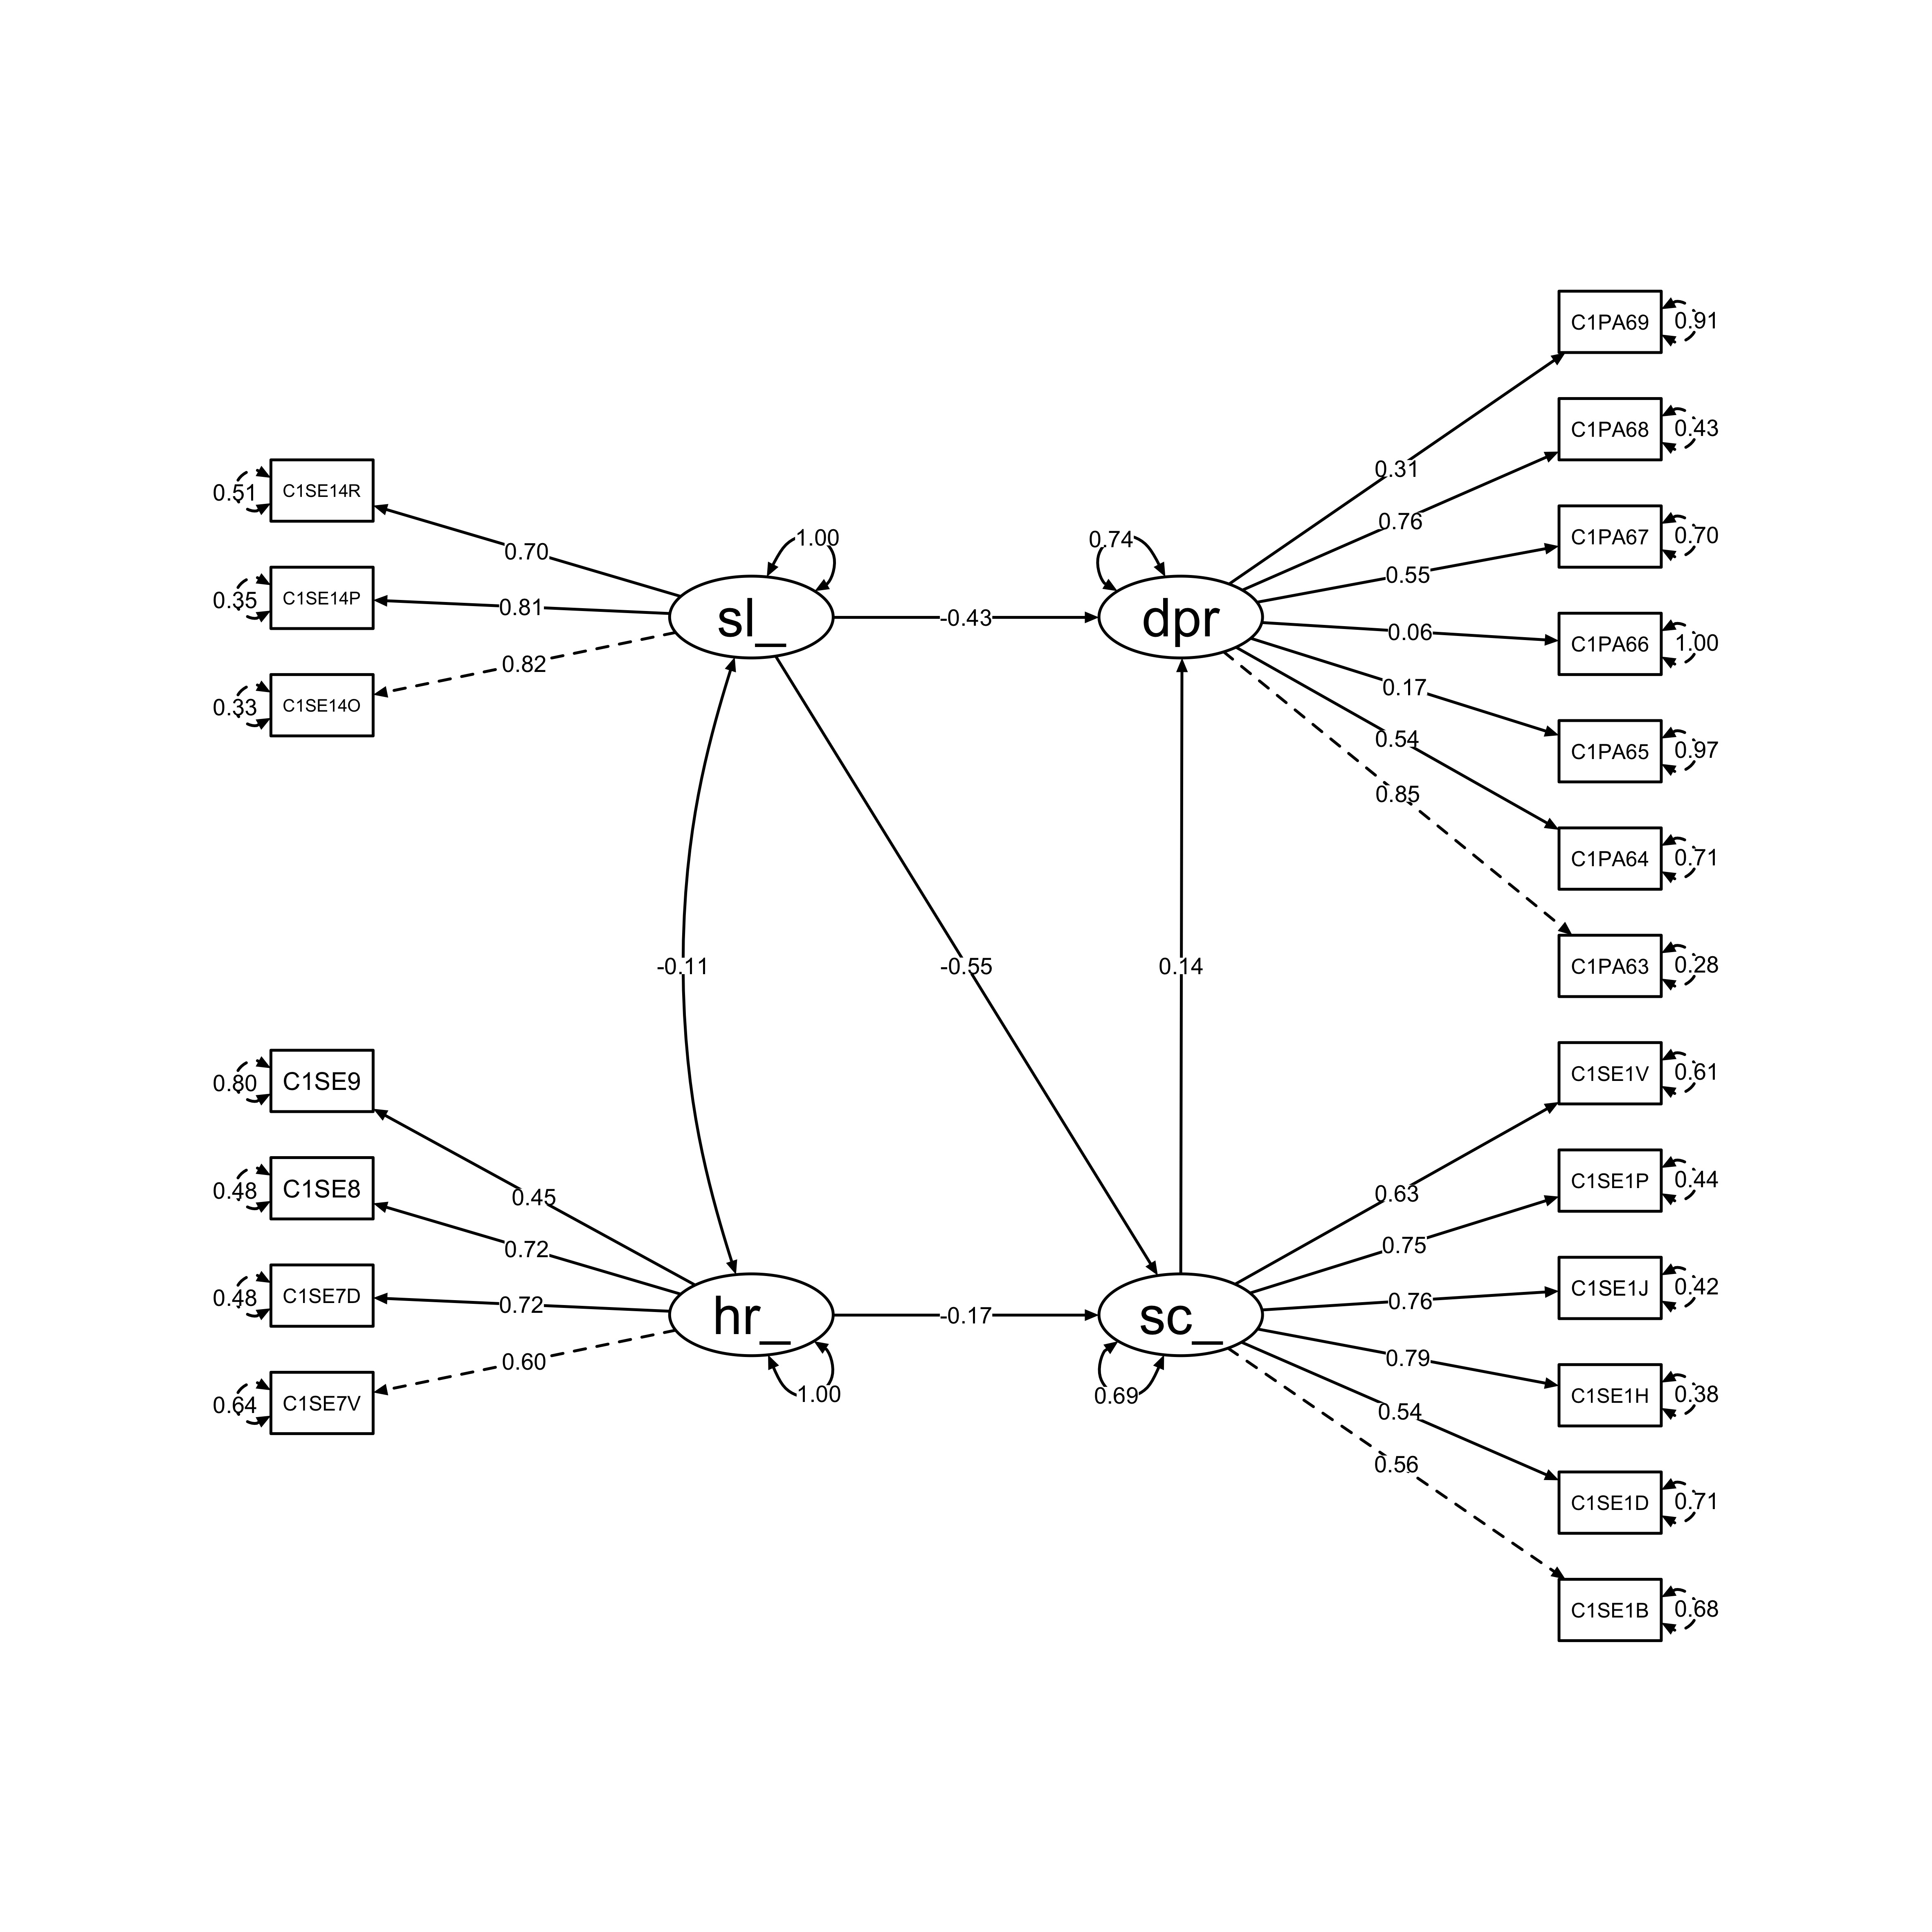
\includegraphics[width=14cm]{../visualizations/base_model.png}
\caption{Summary of base model}
\end{figure}

\FloatBarrier
\pagebreak
\section{Expanding the base model}

\FloatBarrier
\pagebreak
\section{Conclusion}

\end{document}
